\documentclass[12pt,english]{article}

\usepackage{natbib}

\usepackage{graphics,graphicx,dcolumn,bm,fleqn,epic,eepic,float}
\usepackage{amssymb,amsmath,multirow,rotate,rotating,color}
\usepackage[utf8]{inputenc}

\usepackage[english]{babel}
\usepackage{caption}
\usepackage{subcaption}
\usepackage{tikz}
\usepackage{hyperref}
\hypersetup{
    colorlinks=true,
    linkcolor=blue,
    filecolor=magenta,      
    urlcolor=cyan,
}
%\usepackage[usenames,dvipsnames,svgnames,table]{xcolor}
\tikzset{fontscale/.style = {font=\relsize{#1}}}
\usetikzlibrary{calc}
\makeatother

\newcommand{\figref}[1]{Fig.~\ref{fig:#1}}
\newcommand{\eqnref}[1]{Eq.~(\ref{eq:#1})}
\newcommand{\ts}{\textsuperscript}

\definecolor{tuered}{RGB}{214,0,74}

\newcommand{\todo}[1]{\textbf{\textcolor{tuered}{ TODO: #1}}}

\newcommand{\vectornorm}[1]{\left|\left|#1\right|\right|}

\renewcommand{\vec}[1]{\mathbf{#1}}
\newcommand{\uvec}[1]{\hat{\vec{#1}}}
\newcommand{\tensor}[1]{\mathbf{#1}}

\definecolor{pyblue}{HTML}{1F77B4}
\definecolor{pyorange}{HTML}{FF7F0C}
\definecolor{pygreen}{HTML}{2CA02C}
\definecolor{pyred}{HTML}{D62728}

\begin{document}

% The referee PDF has been generated from r239 -- 'make referee' command.

\section*{Reply to Referee two}

We thank the Referee for his/her kind report on our work. 
It is a pleasure to read that he/she finds the work relevant and interesting.
We understand the criticism on section 4 and hope to sort out any unclear and confusing statements. 
In what follows we provide detailed answers to all referee's questions and we discuss all the changes made to the manuscript
(which are typeset in red colour).

\begin{itemize}


\item[ \textbf{\underline{Comment 1.}}]
{
It is not clear to me why the kink in the curves showing the difference of the two drops height (by the way, do we talk about the time when the derivative of $\Delta h$ suddenly decreases?) should coincide with the time at which $h_0$ reaches the precursor film height $h^{\ast}$. 
I have no doubt that equation (26) should hold, but I think figure 5 would benefit from convincing the reader that these kinks correspond indeed to the time for which $h_0$ reaches $h^{\ast}$.
}

\item[ \textbf{Answer}]
{
We are sorry if we were not clear or convincing enough with our statement.
The values of $\Delta h$ can only change due to a flow from one droplet into the other, it is an effective measure for asymmetry.
Fluid that is advected from one droplet into the other has to flow through the bridge $h_0(t)$.
By the time $h_0(t)\approx h^{\ast}$ we have a sizeable restriction on the flow due to the boundary condition equation A9. 
To the best of understanding that is why the slopes in $\Delta h$ change and we have a kink.89
}

\item[ \textbf{\underline{Comment 2.}}]
{
About the inset in figure 5 : Why isn't this curved plotted in log-log?
Moreover, if each point corresponds to a curve in the major plot, it would be better to use the same marker.
}

\item[ \textbf{Answer}]
{
It is indeed odd that we choose a linear inset in study about scaling laws.
Our intention was to show that overlap with equation 26 is significant, even with linear scaled axes.
We are sorry for the inconvenience and agree with the referee's suggestions, see figure~\ref{fig:hdiffandloginset}

\begin{figure}
    \centering
    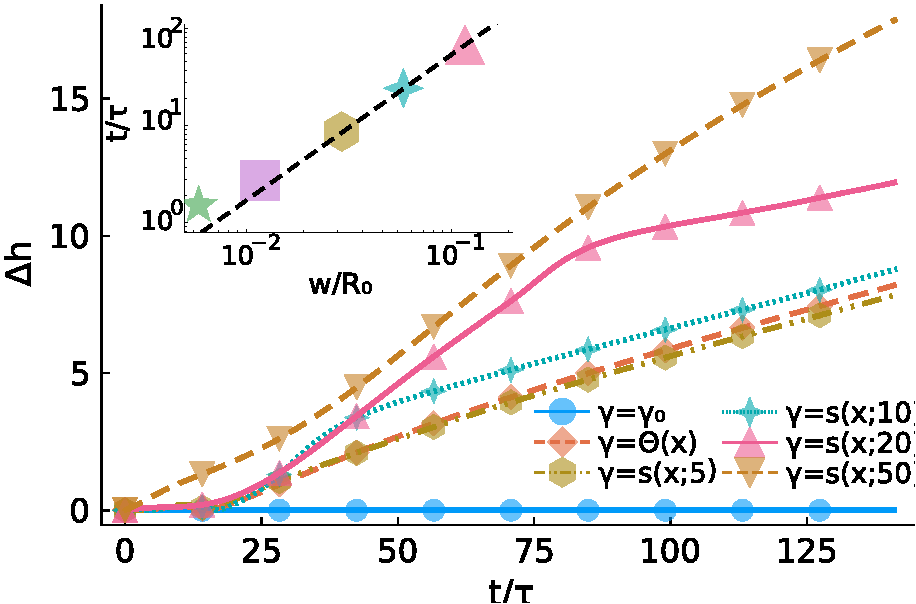
\includegraphics[width=0.85\textwidth]{Figures/h_diff_inset_loglog.pdf}
    \caption{Difference between the maxima of the two droplets.
    In blue, we supply the symmetric coalescence using $\gamma(x) = \gamma_0$.
    The other curves are subject to a surface tension gradient, with different symbols and colors show different $\gamma(x)$.
    The inset displays the droplet separation time (\textcolor{red}{different symbols}) for a subset of \textcolor{red}{$\tanh$-}surface tensions.
    The black dashed line is a power-law $\sim w^{3/2}$.}
    \label{fig:hdiffandloginset}
\end{figure}
}

\item[ \textbf{\underline{Comment 3.}}]
{
It is mentioned at the end of page 4, that the bridge can move. 
Although it seems obvious, could the authors emphasis the fact that they measure $h_0(t)$ at the point of minimum height? 
By the way, shouldn't the analysis be modified in this case, and formulated in a moving frame of reference with a different boundary condition for the velocity at the wall?
}

\item[ \textbf{{Answer}}]
{
The referee is correct in pointing this out and we are sorry for not being clear enough. 
Our protocol for measuring the bridge height is indeed linked to the minimal thickness in between the maxima.
In fact only for $\gamma(x) = \gamma_0$ we observe a stationary bridge in the horizontal dimension.

The imposed boundary condition for the whole substrate is a slip-boundary condition. 
We do 
}

\item[ \textbf{\underline{Comment 4.}}]
{
Could the authors comment on the derivation of equation (24) and give the hypothesis?
}

\item[ \textbf{{Answer}}]
{
\todo{Both referees point this out, damn.}
}


\end{itemize}


\bibliographystyle{abbrv}
\bibliography{Ref}

\end{document}
